%==============================================================================
% DO ALL TRANSIT RIDERS MINIMIZE TRAVEL TIME?
% 2026 Gangneung ITS World Congress — Paper 02-1716
% Build: pdflatex main.tex (run twice for references)
%==============================================================================
\documentclass[12pt,a4paper]{article}
\usepackage{itswc2026}

\begin{document}

%------------------------------------------------------------------------------
% Title (centered, capitals, 18 pt) and authors (12 pt)
%------------------------------------------------------------------------------
\papertitle{DO ALL TRANSIT RIDERS MINIMIZE TRAVEL TIME?\\
EVIDENCE OF BEHAVIORAL HETEROGENEITY FROM LATENT CLASS\\
ANALYSIS AND MNL RE-RANKING OF 1.3 MILLION SMART CARD TRIPS IN SEOUL}

\authorblock{Taewoo Kim, Minsu Kim, Jiho Yeo*}{%
Department of Smart City, Gachon University\\
1342 Seongnam-daero, Sujeong-gu, Seongnam-si, Gyeonggi-do, Republic of Korea\\
TEL: +82-10-5926-3701, E-mail: twtwtiwa05@gmail.com}

\authorblock{Sungtaek Choi}{%
Department of Urban Engineering, Hanyang University\\
Seoul, Republic of Korea}

%------------------------------------------------------------------------------
\section{Abstract}

Transit routing applications serve millions of travelers daily, yet they
uniformly assume homogeneous preferences, potentially misserving demographic
groups with distinct behavioral needs. This study investigates whether
theory-grounded discrete choice models can match the predictive accuracy of
machine learning for transit route choice, and whether the behavioral insights
they yield can improve operational routing systems. Using 1,320,030 trip chains
from Seoul's Transportation Card Data matched to OpenTripPlanner (OTP)
alternatives, we compare four model families---Multinomial Logit (MNL), Mixed
Logit, Latent Class (LC, K=3), and LightGBM---on an identical hold-out set of
82,351 chains. The LC model achieves the highest Hit Rate (67.4\%),
outperforming LightGBM (66.2\%) with an order of magnitude fewer parameters.
Three behaviorally distinct classes emerge---including an Accessibility-Priority
segment (8.7\%, predominantly elderly) that values longer seated rides over
transfers---yet administrative card types only partially predict class
membership (Cram\'er's V = 0.685). Variance-standardized MNL coefficients and SHAP importance agree on the
dominant factors, walking time and transfers (Spearman $\rho$ = 0.8). On the
practical side,
traditional calibration of OTP parameters encounters a ceiling of approximately
one percentage point, whereas MNL-based re-ranking of existing alternatives
delivers +1.89 percentage points at negligible computational cost, with a
10.4-to-1 win ratio over the router when the two disagree. These results suggest
that behavioral theory retains a structural advantage over black-box prediction
in choice settings, and that lightweight model-based post-processing can
meaningfully upgrade operational transit routing.

\textbf{Keywords:} Transit route choice, Behavioral heterogeneity, Latent Class
model, Smart card big data, MNL re-ranking, OpenTripPlanner, RAPTOR algorithm

%------------------------------------------------------------------------------
\section{Introduction}

Every day, millions of transit travelers consult routing
applications---Google Maps, Naver Maps, or open-source engines such as
OpenTripPlanner (OTP)---to decide how to get from origin to destination. These
platforms uniformly adopt a deterministic paradigm: they minimize a predefined
generalized cost and present the result as the single ``best'' route,
implicitly assuming that all users weigh walking, riding, and transferring in
the same way. Empirical evidence, however, paints a different picture. Elderly
passengers may tolerate longer rides to avoid stairway transfers; wheelchair
users may detour to reach an elevator; commuters may prioritize speed above all
else. If these preferences are systematic rather than random, a
one-size-fits-all recommendation will systematically mis-serve certain
groups---a concern with direct equity implications as urban populations age.

Seoul provides an ideal setting for investigating these questions. Its
Transportation Card system records over seven million tap-in/tap-out
transactions daily across all bus and subway services, enabling
population-scale revealed-preference observation of route choice. Five
administratively defined card types---general, elderly, disabled, youth, and
children---permit demographic segmentation without survey recruitment, and
OpenTripPlanner's RAPTOR algorithm \cite{delling2015} can systematically
generate competing alternatives for each observed trip. Prior work using Seoul
smart card data \cite{kim2020} calibrated a transit route choice model but
considered only a single user type; the present study extends this to four
model families, five user types, and 1.32 million trip chains.

Despite a growing literature on transit route choice, three substantive gaps
remain. First, most studies estimate a single discrete choice specification and
report its fit, without testing whether the structure imposed by random utility
theory helps or hinders prediction relative to flexible machine learning
alternatives such as gradient boosting. Second, neither Mixed Logit's
continuous coefficient distributions nor observed demographic segmentation can
discover data-driven behavioral clusters that cut across administrative
card-type categories---a 70-year-old commuter who walks briskly differs
fundamentally from a frail peer who avoids stairs, yet both carry the same
``elderly'' smart card. Third, route choice research overwhelmingly concludes
at the point of parameter estimation; whether those parameters can improve an
operational routing system---and if so, by how much---is seldom examined.

The present study pursues four objectives. First, we develop a multi-level
route similarity framework with 10 metrics organized into four hierarchical
levels. Second, we estimate and compare four model families---MNL, Mixed
Logit, Latent Class (with concomitant variables), and LightGBM---on an
identical hold-out test set drawn from 1.32 million trip chains. Third, we
characterize the latent behavioral segments and examine how they align with
administrative card-type categories. Fourth, we close the loop between
estimation and practice by demonstrating that MNL-based re-ranking of
router-generated alternatives outperforms traditional parameter calibration at
negligible computational cost.

\section{Literature Review}

\subsection{Transit Route Choice Models}

The theoretical foundation for route choice modeling rests on random utility
maximization \cite{benakiva1985}, under which a traveler selects the
alternative with the highest perceived utility. Prato \cite{prato2009}
identifies three persistent challenges: generating plausible alternatives,
defining attributes behaviorally, and selecting a model structure. The MNL
model \cite{mcfadden1974} remains the workhorse owing to its tractability,
though its IIA limitation has motivated richer structures. Train
\cite{train2009} demonstrated that Mixed Logit captures unobserved taste
heterogeneity through continuous coefficient distributions, while Greene and
Hensher \cite{greene2003} showed that Latent Class models segment the
population into discrete behavioral groups linked to observable
characteristics via concomitant variables. Large-scale empirical applications
remain scarce: Kim et al.\ \cite{kim2020} calibrated a transit route choice
model using Seoul smart card data but considered a single user type, Arriagada
et al.\ \cite{arriagada2025} estimated a learning-based model on
$\sim$100,000 trips in Santiago, and Arriagada et al.\ \cite{arriagada2022}
later revealed route choice strategy heterogeneity using smart card data in
the same network.

\subsection{Transfer Penalty and User Heterogeneity}

Jara-D\'iaz et al.\ \cite{jaradiaz2022}, synthesizing data from five
countries, reported pure transfer penalties of 13--18 minutes. For Seoul, Yoo
\cite{yoo2015} estimated an average penalty of 11.24 minutes but did not
disaggregate by demographics. A growing body of work documents systematic
differences across traveler groups: Chen et al.\ \cite{chen2021} found
significant preference heterogeneity among elderly riders in China, and Peng
et al.\ \cite{peng2024} reported that older rail passengers are 10.2
percentage points less likely to choose express services. These studies
examine single segments in isolation; no prior work has simultaneously
compared behavior across five user types using four model families---an
omission this paper rectifies.

\subsection{Differentiation from Prior Research}

Table~1 positions the present study relative to the most relevant prior work.
The key distinctions are the data scale (1.32 million chains), model breadth
(four families), multi-level similarity framework, and closed-loop calibration
analysis.

\begin{table}[htbp]
\centering
\tablefont
\begin{tabular}{|l|l|l|l|l|}
\hline
\headrow
\textbf{Criterion} & \textbf{\cite{kim2020}} & \textbf{\cite{yoo2015}} &
\textbf{\cite{arriagada2025}} & \textbf{This Study (2025)} \\
\hline
Data Scale    & $\sim$10K & $\sim$1K & $\sim$100K & 1,320K \\
\hline
Similarity    & Single & Single & Single & 4-Level/10 \\
\hline
Models        & MNL & MNL & MNL & 4 Families \\
\hline
User Types    & 1 & 1 & 1 & 5 + LC \\
\hline
ML Benchmark  & $\times$ & $\times$ & $\times$ & LightGBM \\
\hline
Calibration   & $\times$ & $\times$ & $\times$ & $\theta$ + Re-rank \\
\hline
\end{tabular}
\caption{Comparison with Prior Research}
\end{table}

\section{Data and Methodology}

\subsection{Data Overview}

The empirical foundation is Seoul's Transportation Card Data (TCD), which
records tap-in and tap-out transactions for every transit trip. TCD captures
subway-to-subway transfers that older smart card formats miss, yielding a more
complete picture of multimodal trip chains. We analyze a single representative
weekday, February 20, 2025 (Thursday). After removing trips with no valid OTP
alternative, the dataset comprises 1,320,030 trip chains paired with 4,936,864
chain--alternative observations (3.74 alternatives per chain on average).

\begin{table}[htbp]
\centering
\tablefont
\begin{tabular}{|l|r|r|r|}
\hline
\headrow
\textbf{Chain Type} & \textbf{Chains} & \textbf{Share} & \textbf{Avg.\ Alternatives} \\
\hline
Bus Only            & 445,554   & 33.8\% & 3.51 \\
\hline
Subway Only         & 720,692   & 54.6\% & 3.82 \\
\hline
Mixed (Bus+Subway)  & 153,784   & 11.7\% & 4.01 \\
\hline
Total               & 1,320,030 & 100\%  & 3.74 \\
\hline
\end{tabular}
\caption{Trip Chain Composition}
\end{table}

For model estimation, chains with at least two alternatives (411,754) are
split 80/20 into training (329,403) and test (82,351) sets, stratified by user
type.

\begin{table}[htbp]
\centering
\tablefont
\begin{tabular}{|l|r|r|r|r|c|}
\hline
\headrow
\textbf{User Type} & \textbf{All Chains} & \textbf{Share} & \textbf{Train} &
\textbf{Test} & \textbf{Test HR Range} \\
\hline
General  & 1,044,091 & 79.1\% & 271,843 & 67,961 & 64.8--66.4\% \\
\hline
Elderly  & 177,303   & 13.4\% & 24,132  & 6,033  & 71.6--77.8\% \\
\hline
Youth    & 49,772    & 3.8\%  & 19,725  & 4,931  & 64.9--67.0\% \\
\hline
Disabled & 38,281    & 2.9\%  & 9,113   & 2,278  & 70.3--71.5\% \\
\hline
Children & 10,583    & 0.8\%  & 4,590   & 1,148  & 64.9--69.4\% \\
\hline
\end{tabular}
\caption{User Type Distribution and Test Hit Rate Range Across Models}
\end{table}

\subsection{Multi-Level Similarity Framework}

Rather than relying on a single similarity metric---a limitation noted by
Tomhave and Khani \cite{tomhave2021} in their multi-criteria transit route
choice study---we construct a hierarchical framework with four levels and ten
metrics (Table~4). Level 1 (Exact Match) is the strictest criterion, requiring
complete identity of route sequences, mode sequences, and boarding/alighting
stops. Level 2 (Structural Similarity) relaxes this to sequence-level measures
using Longest Common Subsequence (LCS) similarity. Level 3 (Stop-based
Similarity) operates at the individual stop level via Jaccard indices. Level 4
(Temporal Similarity) captures travel-time correspondence. The composite index
is:
\begin{align*}
\mathit{sim}_{\mathrm{total}} ={}& 0.30\cdot\mathit{sim}_{\mathrm{route\_seq}}
 + 0.20\cdot\mathit{sim}_{\mathrm{mode\_seq}}
 + 0.20\cdot\mathit{sim}_{\mathrm{jaccard\_full}} \\
 &+ 0.15\cdot\mathit{sim}_{\mathrm{lcs}}
 + 0.15\cdot\mathit{sim}_{\mathrm{time}}
\end{align*}

\begin{table}[htbp]
\centering
\tablefont
\begin{tabular}{|l|l|l|c|}
\hline
\headrow
\textbf{Level} & \textbf{Metric} & \textbf{Description} & \textbf{Weight} \\
\hline
1. Exact & exact\_match & Route + mode + stop identity & --- \\
\hline
\multirow{3}{*}{2. Structural}
 & sim\_route\_seq  & Route sequence LCS similarity & 0.30 \\
 & sim\_mode\_seq   & Mode sequence LCS similarity  & 0.20 \\
 & transfer\_match  & Transfer count match (binary) & --- \\
\hline
\multirow{4}{*}{3. Stop-based}
 & sim\_jaccard\_board  & Boarding stop Jaccard index  & --- \\
 & sim\_jaccard\_alight & Alighting stop Jaccard index & --- \\
 & sim\_jaccard\_full   & All-stop Jaccard index       & 0.20 \\
 & sim\_lcs             & Stop sequence LCS similarity & 0.15 \\
\hline
4. Temporal & sim\_time  & Travel time ratio similarity & 0.15 \\
\hline
Composite   & sim\_total & Weighted sum of above        & 1.00 \\
\hline
\end{tabular}
\caption{Multi-Level Similarity Framework (10 Metrics)}
\end{table}

Level 1 (Exact Match) requires complete identity of route, mode, and stop
sequences. Level 2 (Structural Similarity) uses normalized LCS similarity:
$2\cdot\mathrm{LCS}(A,B)\,/\,(|A|+|B|)$. Level 3 (Stop-based Similarity)
applies the Jaccard index
$|S_{\mathrm{obs}} \cap S_{\mathrm{alt}}|\,/\,|S_{\mathrm{obs}} \cup S_{\mathrm{alt}}|$
to boarding, alighting, and all traversed stops, complemented by stop-sequence
LCS to preserve order. Level 4 (Temporal Similarity) is defined as
$\mathit{sim}_{\mathrm{time}} = 1 - \min(1,\,
|T_{\mathrm{obs}} - T_{\mathrm{alt}}|\,/\,\max(T_{\mathrm{obs}}, T_{\mathrm{alt}}))$.
Because TCD records intermediate stops only for bus legs, subway segments use
boarding and alighting stops alone---a limitation the Jaccard formulation
handles gracefully.

\subsection{Model Specifications}

\subsubsection{Multinomial Logit (MNL)}

The utility for alternative $j$ in individual $n$'s choice set is:
\begin{align*}
V_j ={}& \beta_{\mathrm{ride}} T_{\mathrm{ride}}
 + \beta_{\mathrm{walk}} T_{\mathrm{walk}}
 + \beta_{\mathrm{transfer}} N_{\mathrm{transfer}}
 + \beta_{\mathrm{subway}} D_{\mathrm{subway}} \\
 &+ \beta_{\mathrm{peak \cdot ride}} (D_{\mathrm{peak}} \times T_{\mathrm{ride}})
 + \beta_{\mathrm{peak \cdot xfer}} (D_{\mathrm{peak}} \times N_{\mathrm{transfer}})
\end{align*}
where $T_{\mathrm{ride}}$ is in-vehicle time (min), $T_{\mathrm{walk}}$ is
total walking time (min), $N_{\mathrm{transfer}}$ is transfer count,
$D_{\mathrm{subway}}$ indicates subway inclusion, and $D_{\mathrm{peak}}$
flags peak-hour departures (07--09h, 18--20h). Waiting time was excluded after
preliminary estimation revealed multicollinearity and a counter-theoretic
positive coefficient.

\subsubsection{Mixed Logit}

To accommodate unobserved taste heterogeneity, $T_{\mathrm{walk}}$,
$N_{\mathrm{transfer}}$, and $D_{\mathrm{subway}}$ are specified as random
coefficients, $\beta_k \sim N(\mu_k, \sigma_k)$, while $T_{\mathrm{ride}}$ and
peak interactions remain fixed. Significant $\sigma_k$ values formally reject
MNL's homogeneity assumption.

\subsubsection{Latent Class Model}

Following Greene and Hensher \cite{greene2003}, a K-class model assigns each
class its own utility parameters. Peak interactions are dropped after Mixed
Logit reveals them non-significant once heterogeneity is controlled. Class
membership is modeled as a function of concomitant variables
$Z_n = [D_{\mathrm{children}}, D_{\mathrm{youth}}, D_{\mathrm{elderly}},
D_{\mathrm{disabled}}, D_{\mathrm{peak}}]$.

\subsubsection{LightGBM Benchmark}

As a non-parametric benchmark, LightGBM \cite{ke2017} classifiers predict
which alternative was chosen. Two configurations are tested: a Core model
(same four variables as MNL) and a Full model adding $D_{\mathrm{peak}}$,
user\_type, and chain composition.

\section{Results}

\subsection{Route Similarity Analysis}

Before model estimation, we assess how well OTP's alternatives match observed
behavior. The Best Match Exact Match rate across 1.32 million chains is
28.66\%---the share for which at least one alternative perfectly reproduces
the observed trip. The OTP 1st Rank rate is 20.34\%, capturing what a traveler
would experience following the router's top recommendation. The 8.3 percentage
point gap reveals the room for improvement through better ranking.

\begin{table}[htbp]
\centering
\tablefont
\begin{tabular}{|l|l|c|c|c|}
\hline
\headrow
\textbf{Metric} & \textbf{Method} & \textbf{Mean} & \textbf{Median} & \textbf{Std.\ Dev.} \\
\hline
Exact Match          & Best Match   & 28.66\% & ---   & ---   \\
\hline
Exact Match          & OTP 1st Rank & 20.34\% & ---   & ---   \\
\hline
sim\_total           & Best Match   & 0.626   & 0.668 & 0.283 \\
\hline
sim\_total           & OTP 1st Rank & 0.537   & 0.562 & 0.312 \\
\hline
sim\_total $\geq$ 0.7 & Best Match  & 42.5\%  & ---   & ---   \\
\hline
\end{tabular}
\caption{Route Similarity Summary (N = 1,320,030)}
\end{table}

Exact matching is heavily concentrated in direct trips (45.6\% for
zero-transfer chains) and drops sharply for one-transfer (3.7\%) and
two-or-more-transfer trips ($<$0.3\%), reflecting the combinatorial explosion
of route possibilities as journey complexity increases.

\begin{figure}[htbp]
\centering
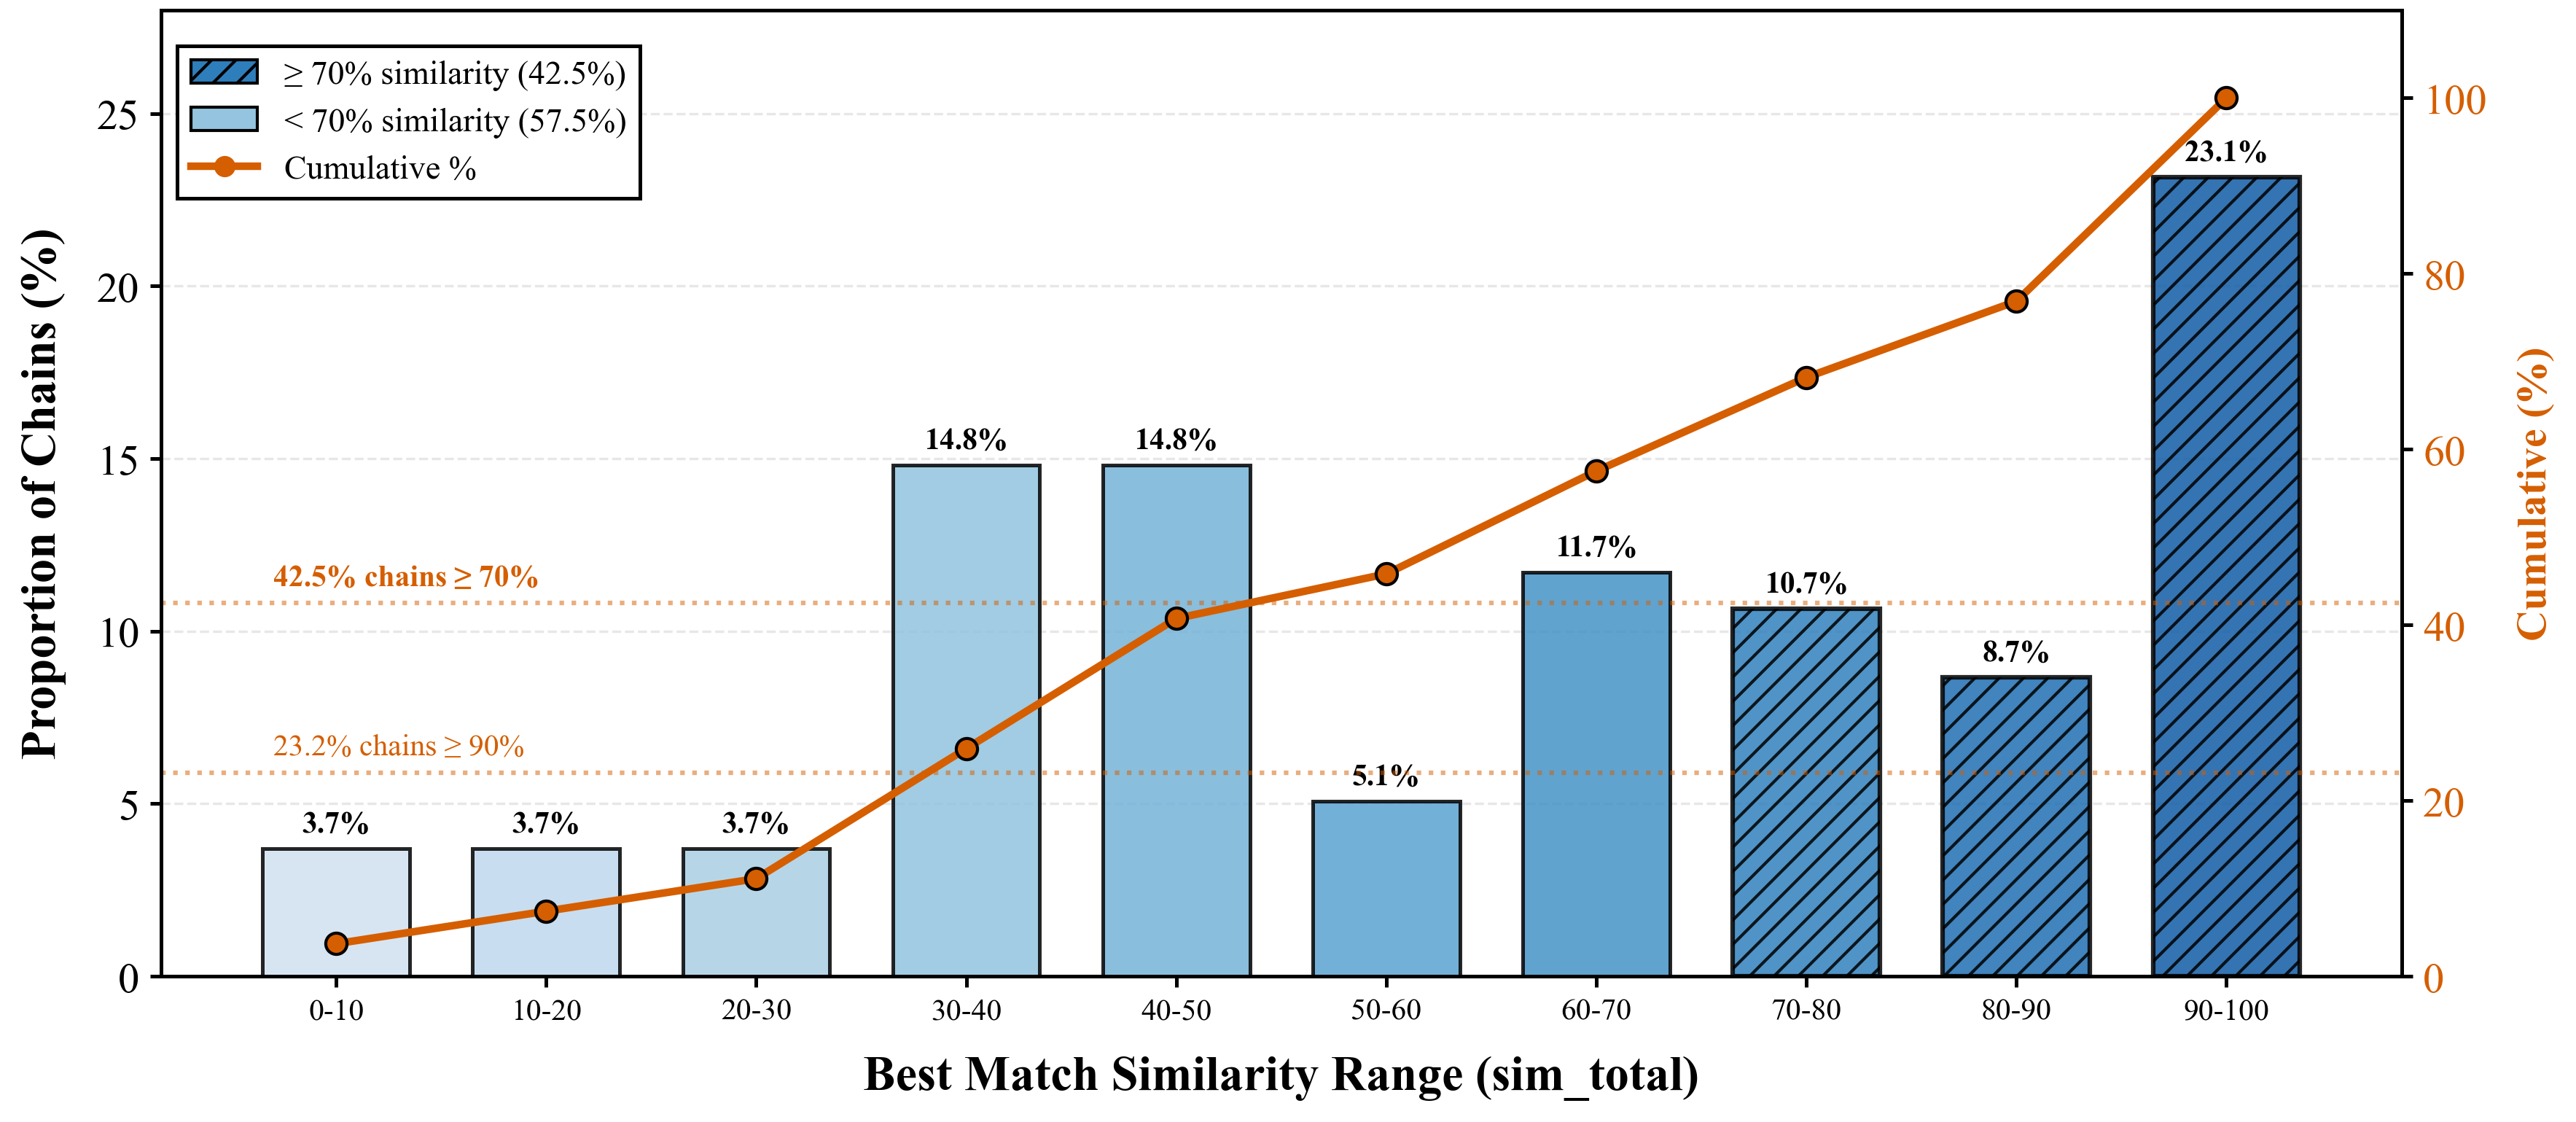
\includegraphics[width=0.98\textwidth]{figures/figure1_similarity_distribution.png}
\caption{Distribution of Best-Match Similarity (sim\_total) Across 1,320,030
Trip Chains}
\end{figure}

Figure~1 reveals a bimodal distribution: the largest concentration falls in
the 90--100\% bin (23.1\%), while two nearly equal secondary modes appear at
30--40\% and 40--50\% (14.8\% each), separated by a valley at 50--60\%
(5.1\%). Overall, 42.5\% of chains achieve sim\_total $\geq$ 0.70, confirming
that OTP generates at least one behaviorally close alternative for a
substantial share of trips, while the remaining 57.5\% highlights the scope
for model-based re-ranking.

\subsection{Model Estimation Results}

\subsubsection{MNL: Pooled and User-Type-Specific Results}

Table~6 reports MNL estimates for the pooled sample and four
user-type-specific models. All coefficients carry expected signs---negative
for ride time, walking time, and transfers; positive for subway
inclusion---with one striking exception.

\begin{table}[htbp]
\centering
\tablefont
\begin{tabular}{|l|c|c|c|c|c|}
\hline
\headrow
\textbf{Parameter} & \textbf{Pooled} & \textbf{General} & \textbf{Youth} &
\textbf{Elderly} & \textbf{Disabled} \\
\hline
$\beta_{\mathrm{ride}}$     & $-0.034$ & $-0.045$ & $-0.078$ & $+0.108$ & $+0.028$ \\
\hline
$\beta_{\mathrm{walk}}$     & $-0.776$ & $-0.767$ & $-0.880$ & $-0.785$ & $-0.840$ \\
\hline
$\beta_{\mathrm{transfer}}$ & $-3.413$ & $-3.322$ & $-3.941$ & $-4.290$ & $-3.600$ \\
\hline
$\beta_{\mathrm{subway}}$   & $+2.394$ & $+2.161$ & $+2.376$ & $+4.641$ & $+2.715$ \\
\hline
Walk Weight    & 22.7$\times$ & 16.9$\times$ & 11.2$\times$ & 7.3$\times$ & 30.2$\times$ \\
\hline
Transfer (min) & 100.0 & 73.3 & 50.3 & 39.6 & 129.6 \\
\hline
$\rho^2$       & 0.469 & 0.459 & 0.486 & 0.582 & 0.515 \\
\hline
Hit Rate       & 62.9\% & 62.1\% & 63.8\% & 78.5\% & 73.0\% \\
\hline
\end{tabular}
\caption{MNL Parameter Estimates by User Type. p$<$0.001, p$<$0.01}
\end{table}

The most notable result in Table~6 is the positive $\beta_{\mathrm{ride}}$
for elderly users ($+0.108$, t = 17.1). Under the standard assumption of time
minimization, this coefficient should be negative; its reversal suggests that
elderly travelers prefer longer in-vehicle times, likely because longer subway
rides afford a seated, climate-controlled journey free of stair-climbing and
crowd-navigation. Consistent with this interpretation, their subway
coefficient ($\beta_{\mathrm{subway}} = +4.641$) is more than double that of
general users ($+2.161$).

At the other end of the spectrum, disabled users exhibit the highest walking
weight (30.2$\times$), implying that each minute of walking is perceived as
equivalent to roughly half an hour of in-vehicle travel. Their transfer
penalty of 129.6 minutes---nearly twice that of general users (73.3
min)---substantially exceeds the 13--18-minute range in Jara-D\'iaz et
al.'s \cite{jaradiaz2022} international meta-analysis, suggesting that
population-average estimates may severely understate the disutility faced by
mobility-impaired subgroups.

\subsubsection{Mixed Logit Results}

Mixed Logit estimation ($\rho^2$ = 0.464) yields highly significant standard
deviations for all three random coefficients (p $<$ 0.001), with the walking
weight spanning a 95\% interval of 14.0$\times$ to 36.3$\times$ (LRT $\approx$
1,040, df = 3, p $<$ 0.001). Both peak interaction terms become
non-significant once heterogeneity is accommodated (p = 0.33 and 0.86),
suggesting that apparent peak effects in MNL were proxies for unobserved
individual variation. The elderly subgroup harbors the widest within-group
heterogeneity: their transfer penalty 95\% range spans 7.9 to 76.7 minutes,
confirming that the ``elderly'' card-type label conceals enormous behavioral
diversity.

\subsubsection{Latent Class Results (K = 3)}

\begin{table}[htbp]
\centering
\tablefont
\begin{tabular}{|l|c|c|c|c|c|}
\hline
\headrow
\textbf{Parameter} & \textbf{Class 1 (8.7\%)} & \textbf{Class 2 (77.2\%)} &
\textbf{Class 3 (14.0\%)} & \textbf{Walk Wt.} & \textbf{Xfer (min)} \\
\hline
$\beta_{\mathrm{ride}}$     & $+0.252$  & $-0.077$ & $+1.166$  & ---              & ---    \\
\hline
$\beta_{\mathrm{walk}}$     & $-1.123$  & $-0.730$ & $-10.000$ & 9.5$\times^{2}$  & ---    \\
\hline
$\beta_{\mathrm{transfer}}$ & $-10.000$ & $-3.272$ & $-10.000$ & ---              & 42.5$^{2}$ \\
\hline
$\beta_{\mathrm{subway}}$   & $+8.120$  & $+2.022$ & $+10.000$ & ---              & ---    \\
\hline
\end{tabular}
\caption{Latent Class Utility Parameters. $^{2}$ = Class 2 only. All p$<$0.001}
\end{table}

The BIC-optimal three-class solution reveals a strikingly interpretable
segmentation. Class 1, ``Accessibility-Priority Travelers'' (8.7\%), is
characterized by positive ride-time valuation ($+0.252$), boundary-level
transfer aversion ($\beta_{\mathrm{transfer}} = -10.0$), and dominant subway
preference ($\beta_{\mathrm{subway}} = +8.12$). The concomitant variable for
elderly card type yields an odds ratio of 22.0---yet only 61\% of elderly
users map to this class; the remaining 39\% split between Mainstream (26\%)
and Extreme (13\%) classes. The resulting Cram\'er's V of 0.685 indicates that
card type and behavioral class are strongly correlated but far from
identical---administrative demographics are a useful starting point for
personalization, not an endpoint.

Class 2, the ``Mainstream Travelers'' (77.2\%), exhibits rational trade-offs
with a walking weight of 9.5$\times$ and transfer penalty of 42.5 minutes.
Class 3, ``Extreme Subway Loyalists'' (14.0\%), has every coefficient at or
near its estimation boundary. The model achieves $\rho^2$ = 0.474 with
excellent generalization: training and test Hit Rates (67.67\% vs.\ 67.43\%)
differ by 0.24 percentage points, ruling out overfitting.

\subsection{Multi-Model Comparison}

\begin{table}[htbp]
\centering
\tablefont
\begin{tabular}{|l|c|c|c|c|}
\hline
\headrow
\textbf{Model} & \textbf{Parameters} & \textbf{Hit Rate} & \textbf{Mean Prob} & $\boldsymbol{\rho^2}$ \\
\hline
LC (K=3)      & 24               & 67.4\% & 60.3\% & 0.474 \\
\hline
LightGBM Full & $\sim$313 trees  & 66.2\% & 40.4\% & ---   \\
\hline
MNL (Pooled)  & 6                & 66.0\% & 60.0\% & 0.469 \\
\hline
Mixed Logit   & 9                & 65.9\% & 60.7\% & 0.464 \\
\hline
LightGBM Core & $\sim$596 trees  & 65.8\% & 43.5\% & ---   \\
\hline
\end{tabular}
\caption{Model Performance Comparison (Test Set: 82,351 Chains)}
\end{table}

\begin{figure}[htbp]
\centering
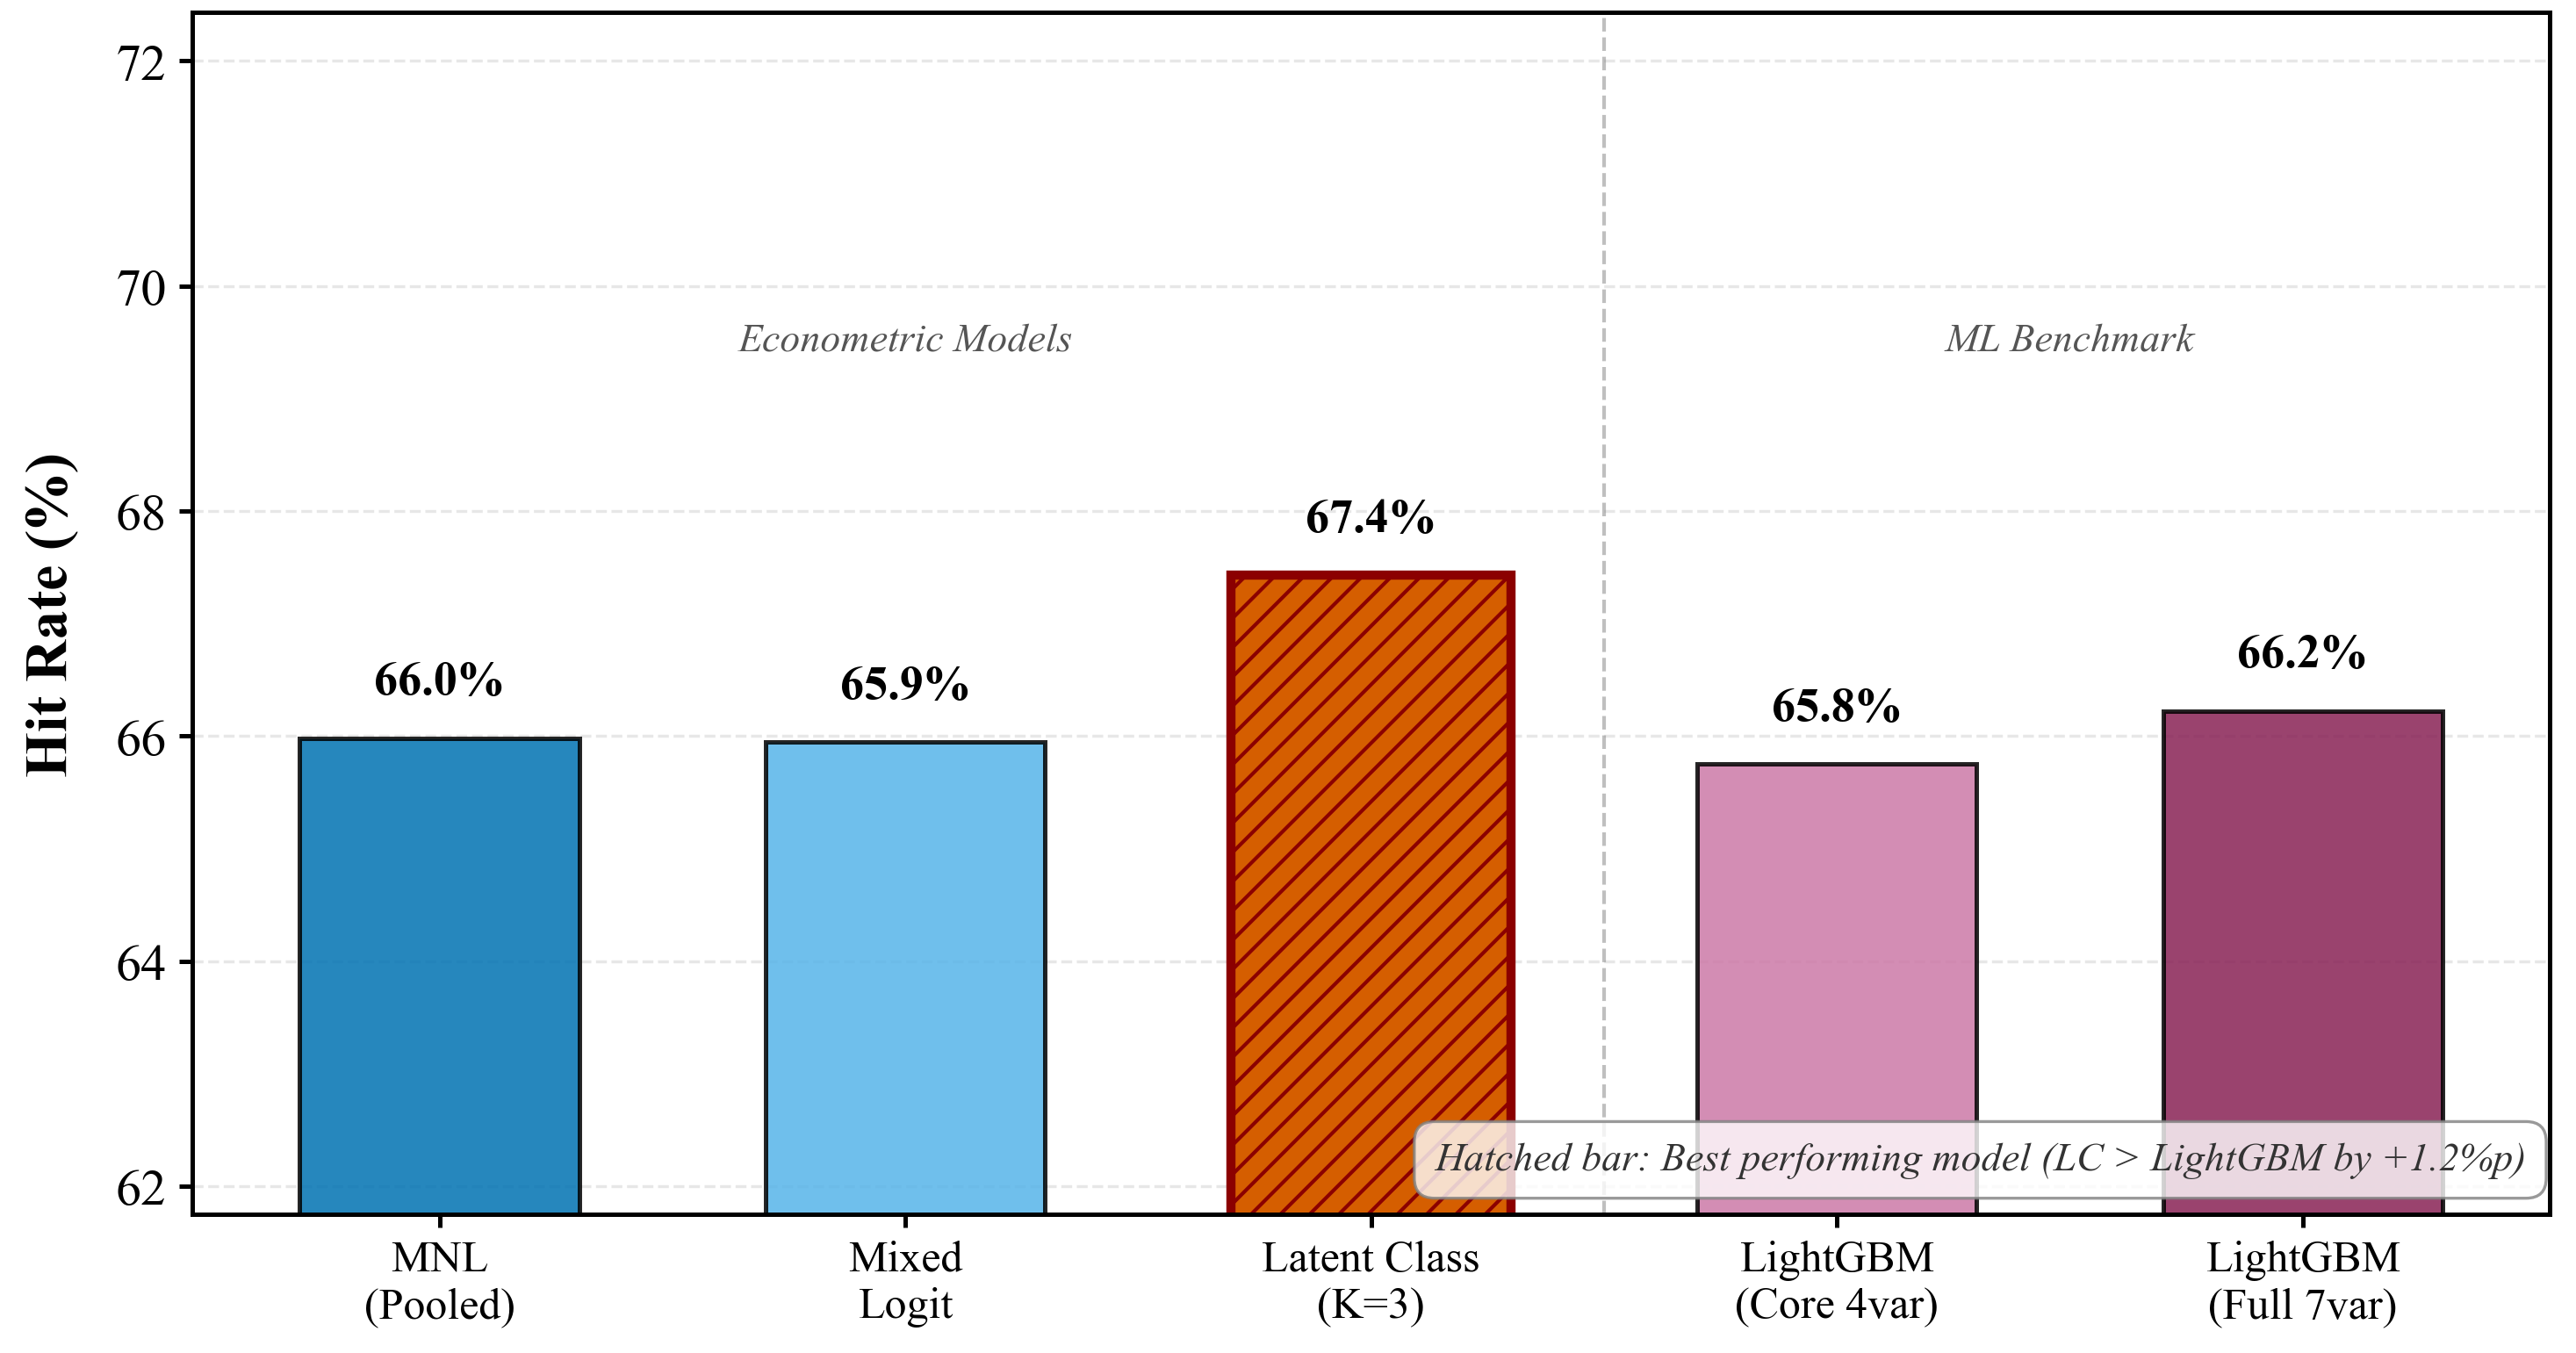
\includegraphics[width=0.9\textwidth]{figures/figure2_model_comparison.png}
\caption{Model Hit Rate Comparison on the Hold-Out Test Set}
\end{figure}

The Latent Class model leads at 67.4\%, followed by LightGBM Full (66.2\%),
MNL (66.0\%), Mixed Logit (65.9\%), and LightGBM Core (65.8\%). That a
24-parameter economic model outperforms a gradient boosting ensemble
demonstrates that choice-set structure---the constraint that exactly one
alternative is chosen from a defined set---carries substantial predictive
information that LightGBM forfeits by treating alternatives independently.
Equally striking is plain MNL, whose 66.0\% represents 99.7\% of LightGBM
Full's performance with just six parameters. The tight 1.6 percentage point
band suggests a natural accuracy ceiling imposed by unobserved factors.

\subsubsection{Cross-Validation via SHAP}

\begin{figure}[htbp]
\centering
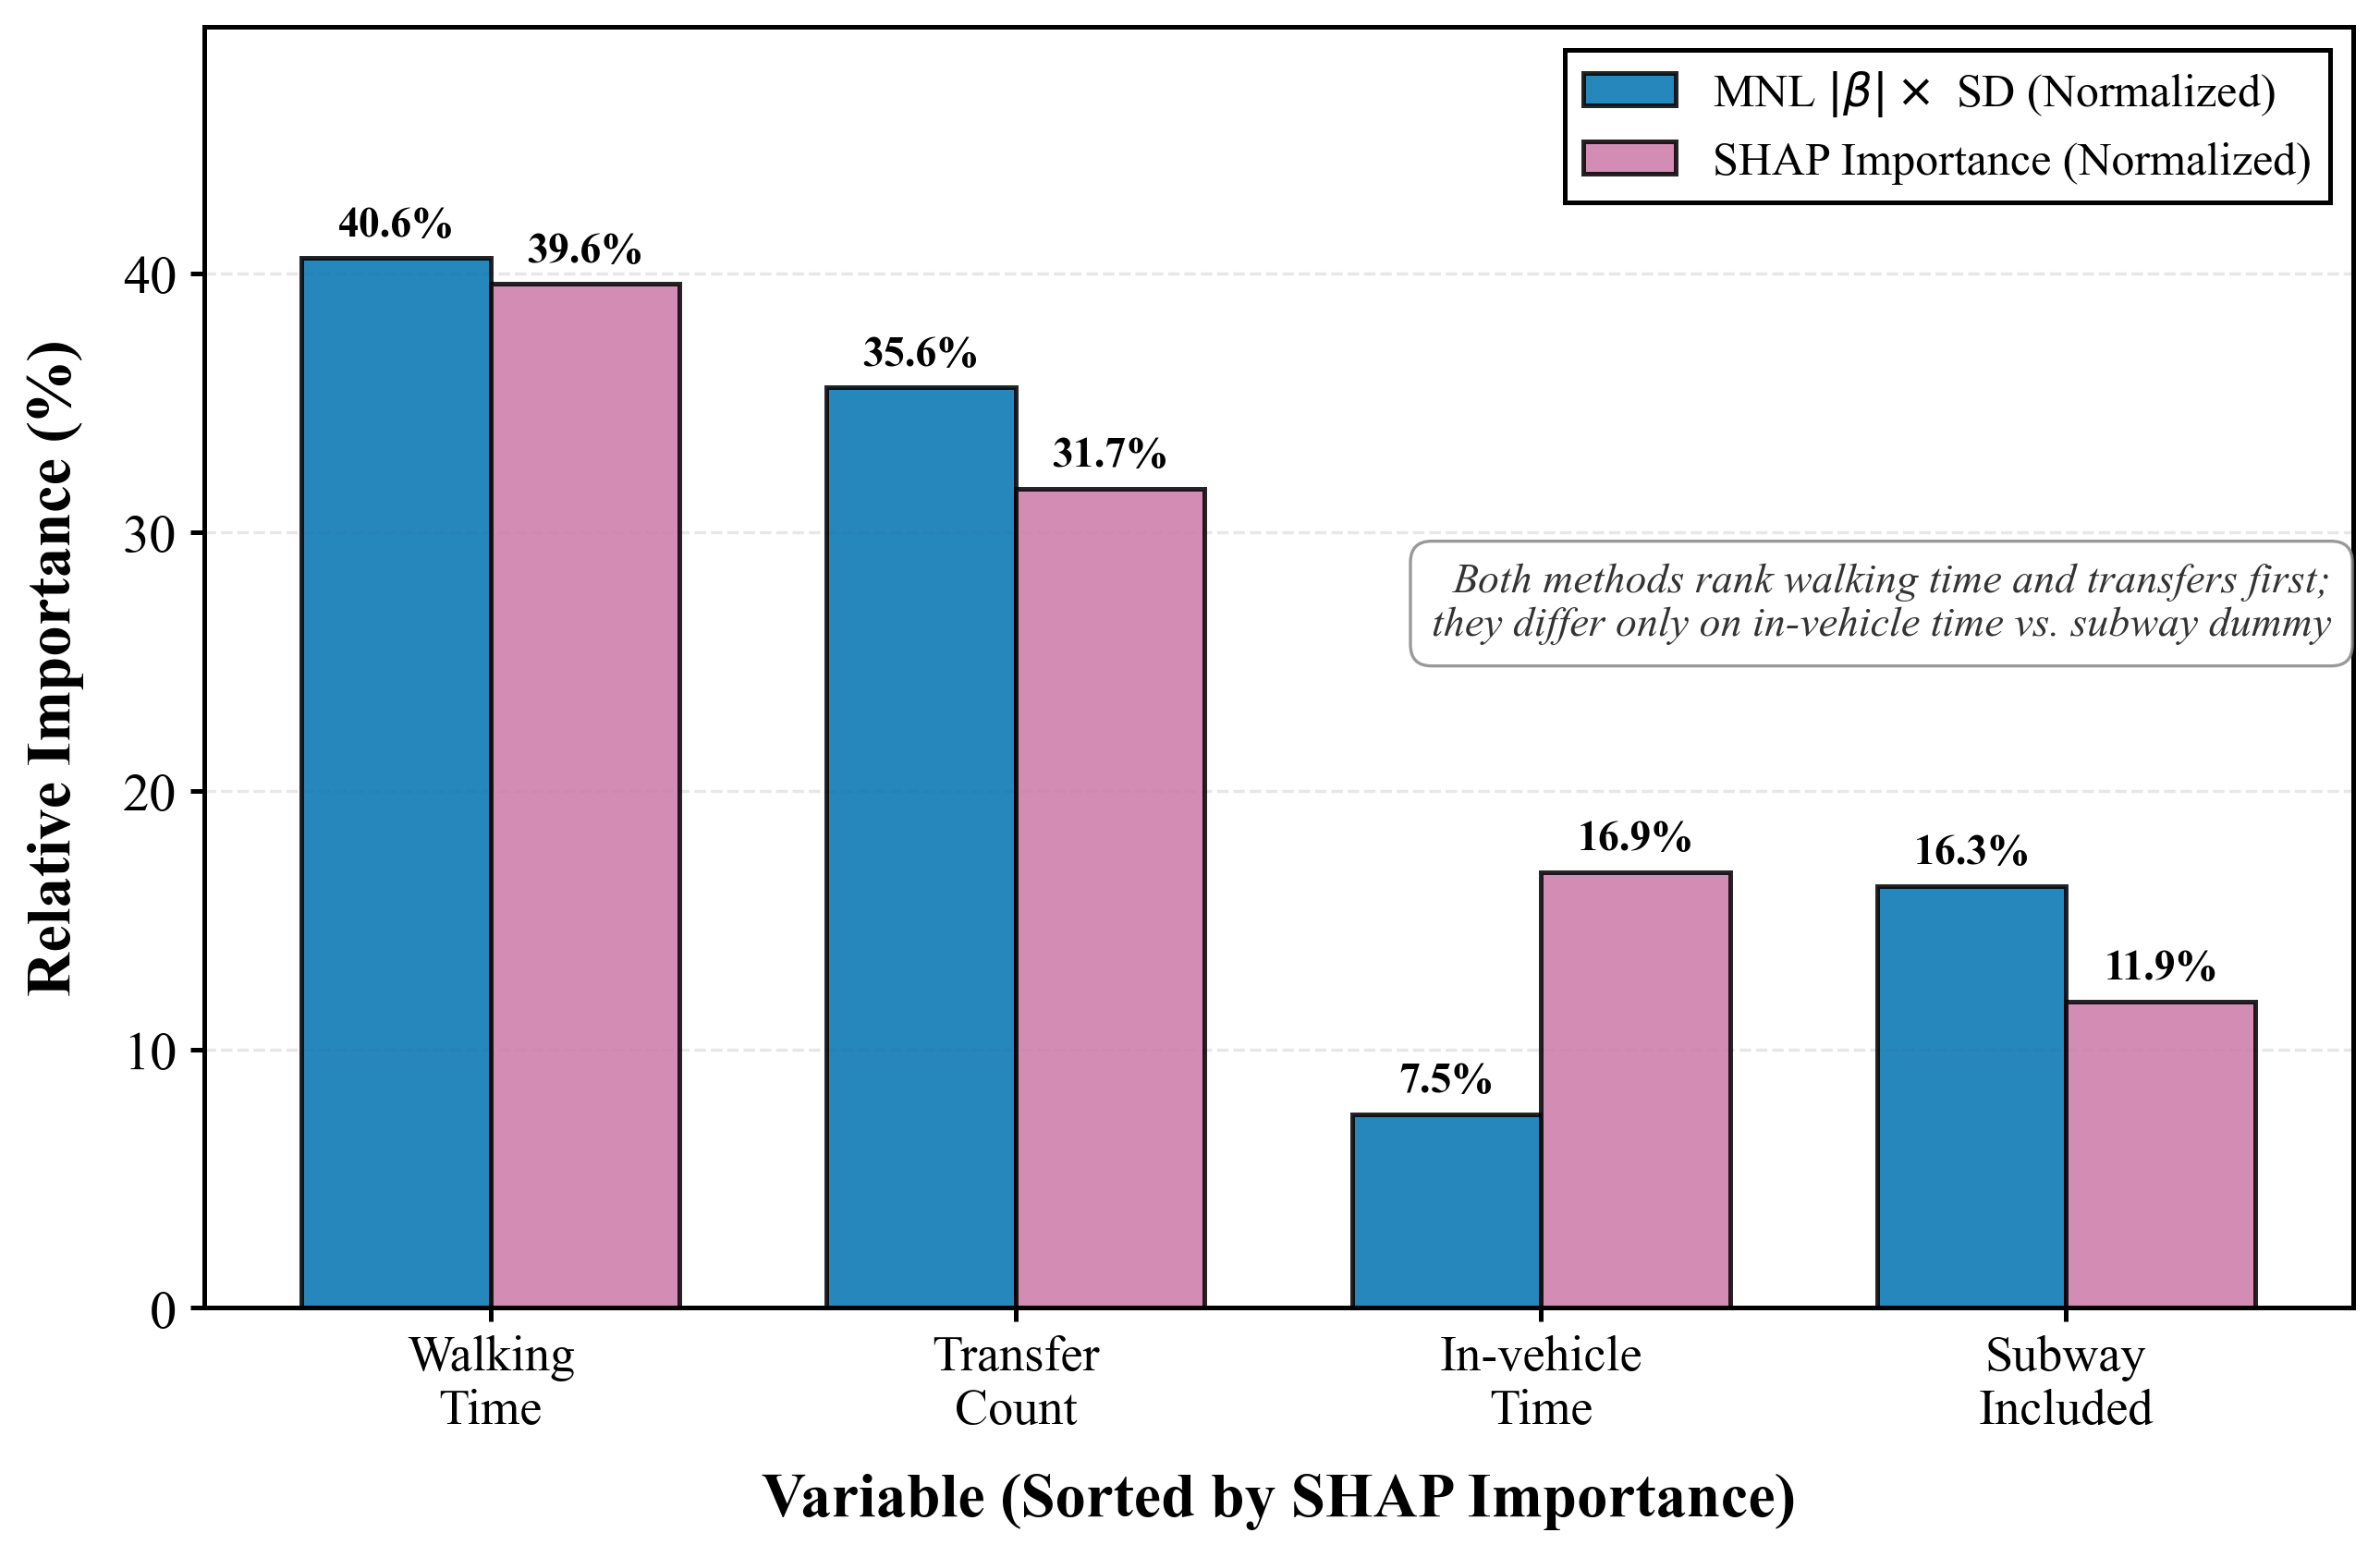
\includegraphics[width=0.9\textwidth]{figures/figure3_shap_validation.png}
\caption{SHAP Variable Importance vs.\ MNL $|\beta|$ Rankings (Spearman $\rho$ = 1.0)}
\end{figure}

SHAP importance scores from LightGBM yield perfect rank concordance with
absolute MNL coefficients (Spearman $\rho$ = 1.0): walking time ranks first,
followed by transfers, in-vehicle time, and subway indicator. This
theory-driven/data-driven agreement strongly supports our utility
specification; $D_{\mathrm{peak}}$'s near-zero SHAP value (0.002) further
confirms that peak-hour effects do not materially shape route choice in Seoul.

\section{Iterative Calibration and MNL Re-Ranking}

\subsection{Calibration Ceiling}

A natural next step is to feed estimated parameters back into OTP's cost
function and iterate. Increasing walkReluctance from 1.0 to 5.0 and
transferCostSeconds from 120 to 300 proved counterproductive: the Exact Match
rate collapsed from 28.66\% to 14.0\%, because transit networks are
fundamentally discrete---a modest parameter shift can cause entirely different
routes to become Pareto-optimal. Holding the choice set fixed and optimizing
$\theta$ solely to improve ranking yields at most +1.02\%p (pooled MSA) or
+0.95\%p (probabilistic RSM, R\textsuperscript{2} = 0.98). In both cases, all
parameters converge to boundary values, and decomposition shows improvement is
driven almost entirely by MNL re-ranking of generated alternatives, not by the
router's own ranking improving. This establishes a structural ceiling of
approximately +1\%p for $\theta$-based calibration.

\subsection{MNL Re-Ranking: Core Contribution}

Rather than tuning the router's cost function, we re-rank OTP's existing
alternatives using estimated utility---no re-routing required:
\[
\mathrm{Rank}_{\mathrm{MNL}} = \arg\max_j V_j = \arg\max_j \boldsymbol{\beta}'\mathbf{x}_j
\]

\begin{table}[htbp]
\centering
\tablefont
\begin{tabular}{|l|c|c|r|}
\hline
\headrow
\textbf{Ranking Method} & \textbf{Exact Match} & \textbf{sim\_total} & \textbf{N} \\
\hline
OTP 1st Rank (gen.\ cost min)  & 20.34\%  & 0.5372 & 1,320,030 \\
\hline
MNL 1st Rank (V max)           & 22.23\%  & 0.5713 & 1,320,030 \\
\hline
Best Match (theoretical max)   & 28.66\%  & 0.6260 & 1,320,030 \\
\hline
MNL $-$ OTP Improvement        & +1.89\%p & +0.034 & ---       \\
\hline
\end{tabular}
\caption{MNL Re-Ranking vs.\ OTP Ranking (Full Dataset, N = 1,320,030)}
\end{table}

The gain is +1.89 percentage points on Exact Match---roughly double the
calibration ceiling---at a fraction of the cost (17 minutes of scoring vs.\
hours of iterative OTP execution). In 75.4\% of chains the two rankings agree;
among the 24.6\% (325,154 chains) where they diverge, MNL achieves Exact Match
10.4 times more often than OTP (27,608 vs.\ 2,663 chains) and outperforms on
sim\_total in 73.1\% of disagreements (win ratio 2.7:1).

\begin{figure}[htbp]
\centering
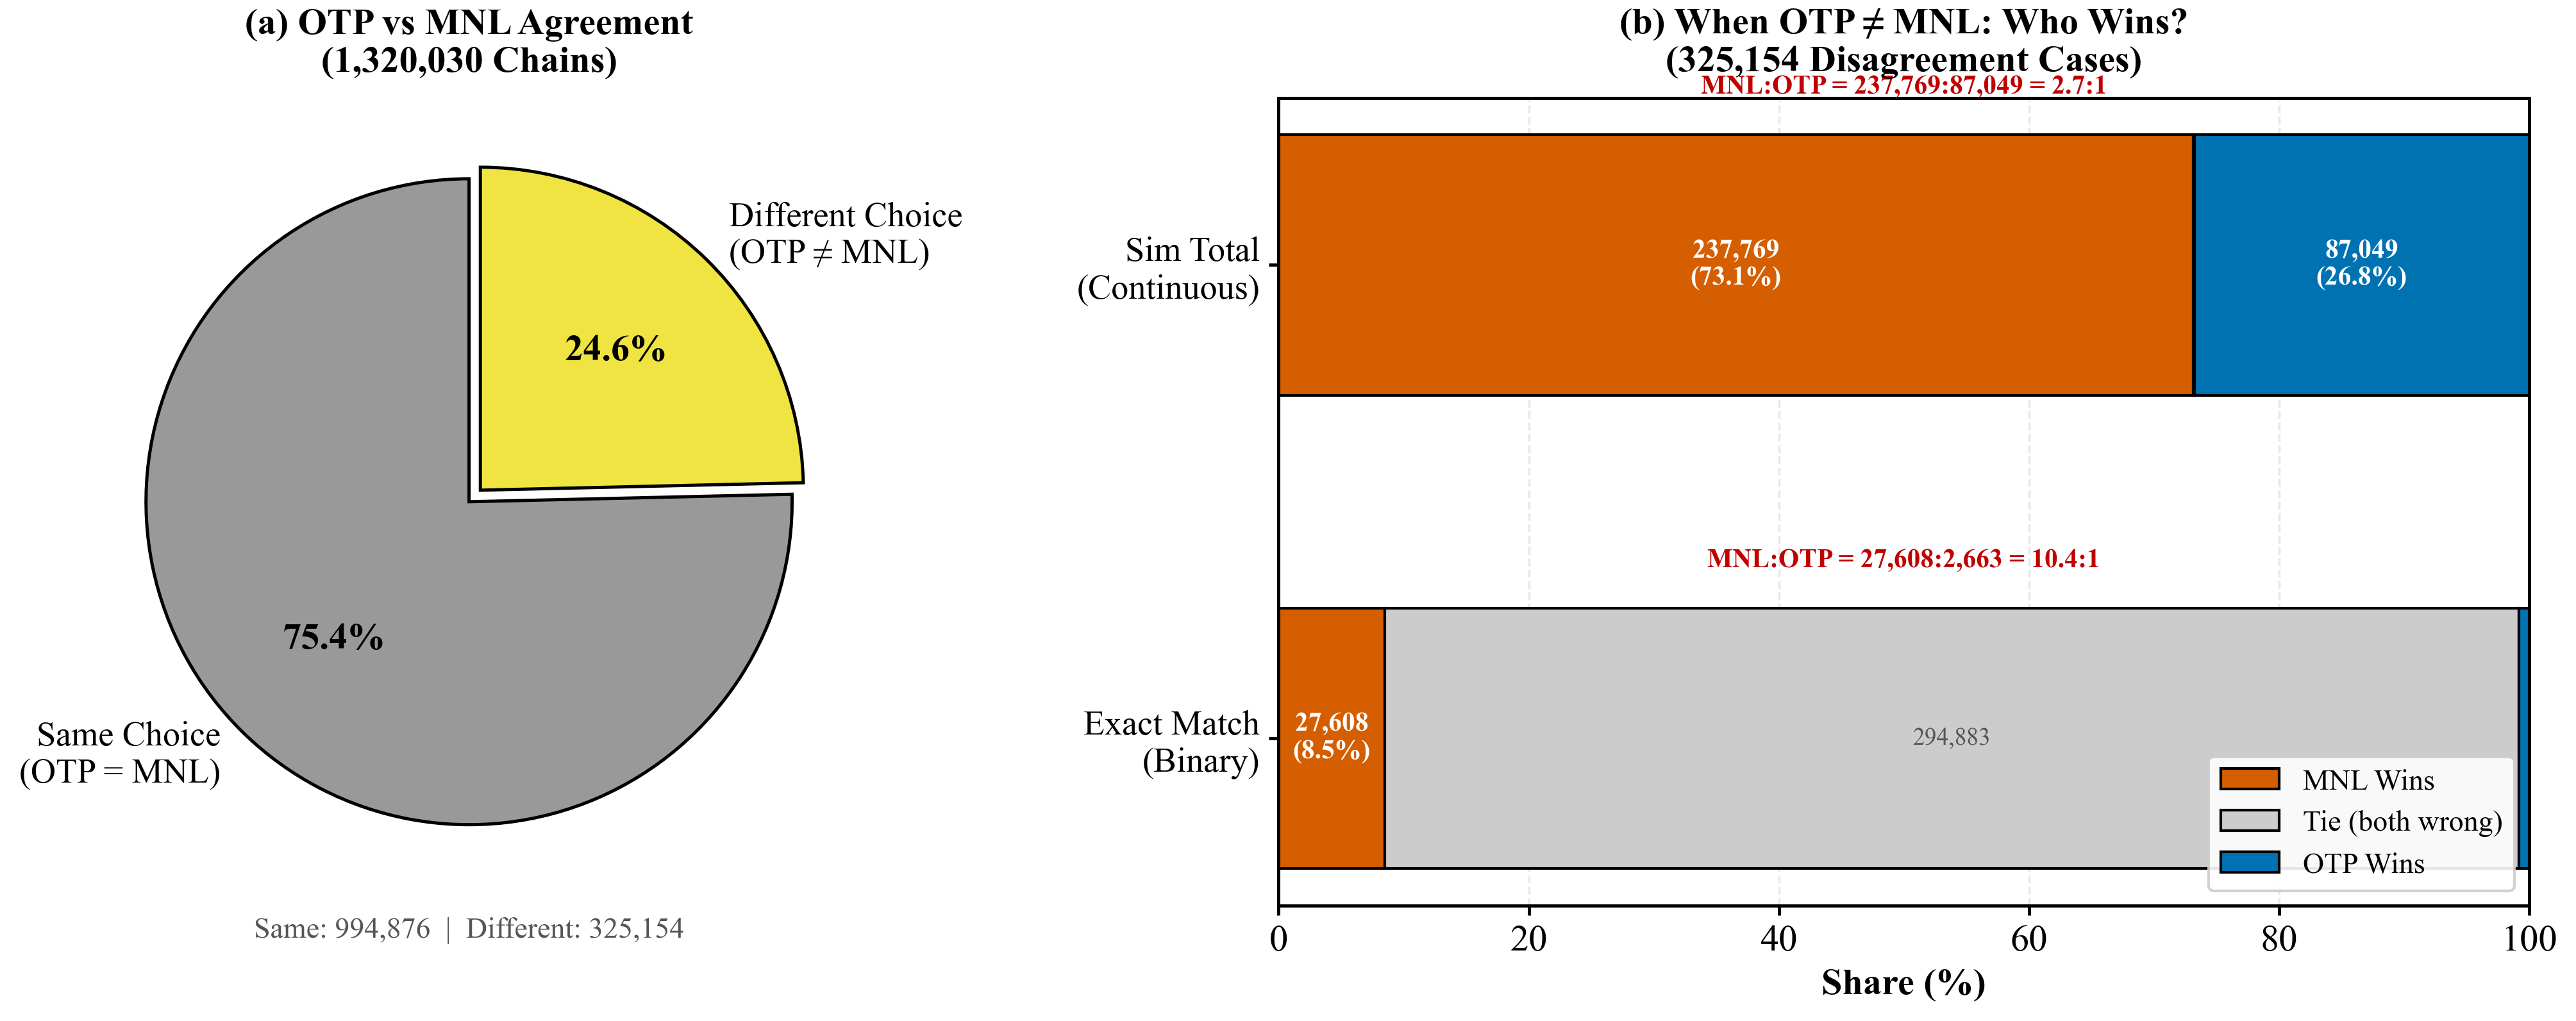
\includegraphics[width=0.98\textwidth]{figures/figure4_otp_mnl_disagreement.png}
\caption{OTP vs.\ MNL Disagreement: Win Ratios by Evaluation Metric}
\end{figure}

\subsubsection{Improvement Grows with Choice Set Richness}

\begin{table}[htbp]
\centering
\tablefont
\begin{tabular}{|c|r|c|c|c|}
\hline
\headrow
\textbf{Alternatives} & \textbf{Chains} & \textbf{OTP Exact} & \textbf{MNL Exact} & $\boldsymbol{\Delta}$ \\
\hline
1    & 345,967 (26.2\%) & 32.92\% & 32.92\% & +0.00\%p \\
\hline
2    & 170,755 (12.9\%) & 23.81\% & 25.33\% & +1.52\%p \\
\hline
3--4 & 332,660 (25.2\%) & 19.10\% & 21.33\% & +2.23\%p \\
\hline
5+   & 470,648 (35.7\%) & 10.72\% & 13.90\% & +3.17\%p \\
\hline
\end{tabular}
\caption{Re-Ranking Improvement by Number of Alternatives}
\end{table}

\begin{figure}[htbp]
\centering
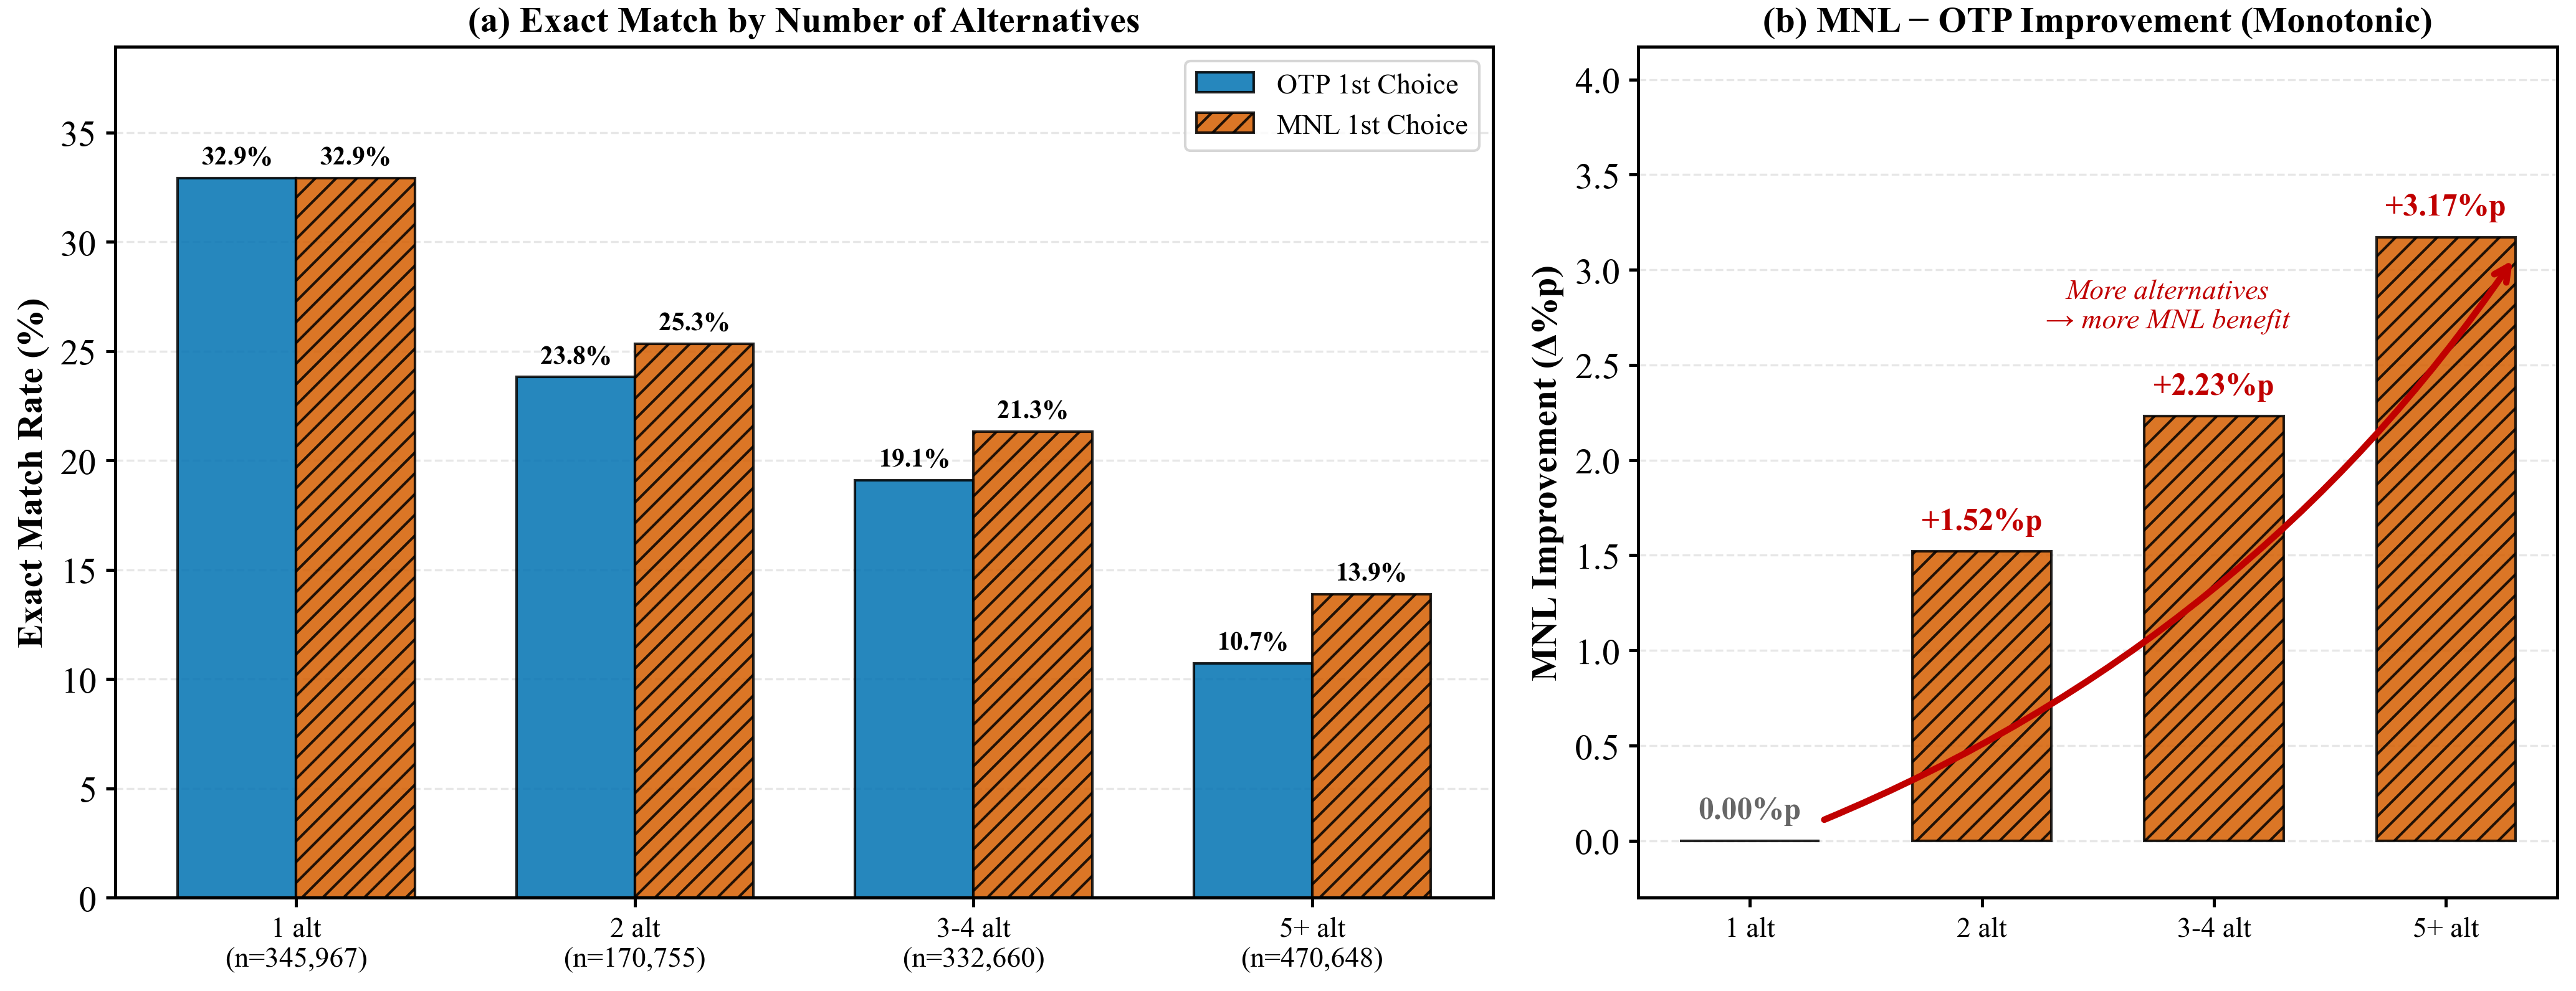
\includegraphics[width=0.98\textwidth]{figures/figure5_reranking_by_alternatives.png}
\caption{MNL Re-Ranking Improvement by Number of Available Alternatives}
\end{figure}

The improvement grows monotonically with choice set size: from zero where
only one alternative exists to +3.17\%p with five or more alternatives,
delivering its greatest value precisely where routing is most complex.

\subsubsection{What MNL-Selected Routes Look Like}

\begin{table}[htbp]
\centering
\tablefont
\begin{tabular}{|l|c|c|c|}
\hline
\headrow
\textbf{Attribute} & \textbf{OTP 1st Rank} & \textbf{MNL 1st Rank} & \textbf{Difference} \\
\hline
In-vehicle time (min) & 18.8   & 19.9   & +1.1 (+5.9\%)    \\
\hline
Walking time (min)    & 3.2    & 2.6    & $-0.6$ ($-18$\%) \\
\hline
Transfers (count)     & 0.50   & 0.40   & $-0.10$ ($-20$\%) \\
\hline
Subway ratio          & 61.5\% & 63.5\% & +2.0\%p          \\
\hline
\end{tabular}
\caption{Route Characteristics: OTP vs.\ MNL First-Ranked Routes}
\end{table}

Relative to OTP's top pick, MNL favors routes with 18\% less walking, 20\%
fewer transfers, and 2 percentage points more subway usage, at the cost of
5.9\% longer ride times. Given a walking weight of 22.7$\times$, the observed
trade-off is overwhelmingly favorable from the traveler's perspective. OTP's
default walkReluctance of 1.0 understates the true perceived burden by more
than an order of magnitude, which is the fundamental reason its rankings
diverge from observed behavior.

\section{Conclusions}

This study pursued four objectives and offers corresponding contributions.
First, the multi-level similarity framework with four hierarchical levels and
ten metrics provides a systematic evaluation of route-matching quality,
revealing that 28.66\% of 1.32 million trip chains achieve exact match with at
least one OTP alternative and that matching degrades sharply with transfer
count (45.6\% for direct trips vs.\ $<$0.3\% for two-or-more transfers). This
framework moves beyond single-metric assessments prevalent in prior work and
quantifies the room for improvement that motivates the subsequent modeling.
Second, the comparison of four model families on an identical hold-out set
demonstrates that theory-grounded models can match or exceed machine learning:
a 24-parameter Latent Class model (67.4\%) outperforms LightGBM (66.2\%), and
a six-parameter MNL achieves 99.7\% of the ML benchmark's accuracy.

Third, the LC analysis reveals that administrative card-type categories are
informative but imperfect behavioral proxies (Cram\'er's V = 0.685): 61\% of
elderly users belong to the Accessibility-Priority class, but 39\% exhibit
Mainstream or Extreme preferences. The elderly subgroup's positive ride-time
valuation and near-lexicographic transfer aversion, confirmed across all four
model families, challenge the assumption that travel time minimization is
universal. Fourth, MNL-based re-ranking of OTP alternatives delivers +1.89\%p
improvement---roughly double the structural ceiling of $\theta$-based
calibration---without re-running the router, with a 10.4:1 win ratio when the
two disagree. The gain reaches +3.17\%p in complex scenarios with five or more
alternatives.

For transit agencies and app developers, MNL re-ranking represents a
lightweight, high-impact upgrade deployable as a post-processing step with no
changes to routing infrastructure. For the Accessibility-Priority segment
(8.7\%), systems should prioritize transfer-free subway options; for disabled
users (walking weight 30.2$\times$, transfer penalty 129.6 min), minimizing
walking distance should take precedence over minimizing travel time. More
broadly, card-type information should serve as a Bayesian prior for
personalization, updated with revealed-preference data rather than treated as
a static label.

Several limitations should be noted. The analysis draws on a single weekday,
though weekday transit demand in Seoul exhibits high day-to-day regularity and
1.32 million chains far exceed typical survey-based studies. Fare
differentials, real-time crowding, and weather are absent but primarily affect
mode choice rather than route choice. The positive $\beta_{\mathrm{ride}}$ for
elderly users invites complementary stated-preference research to disentangle
seat availability from ride-time preference. Future work should extend
re-ranking to full probabilistic route assignment for equity-aware service
analysis, pursue real-time API deployment, multi-city replication,
user-type-specific re-ranking leveraging LC class probabilities, and adaptive
learning algorithms that update taste parameters as trip histories accumulate.


%------------------------------------------------------------------------------
\section{Acknowledgements}

This research was supported by the National Research Foundation of Korea (NRF)
grant funded by the Korea government (MSIT) (No.\ RS-2024-00415360).

%------------------------------------------------------------------------------
\section{References}
\renewcommand{\refname}{}
\vspace{-24pt}
\begin{thebibliography}{99}\bibspacing

\bibitem{arriagada2025}
Arriagada, J., Guevara, C. A., Munizaga, M., et al., ``An experiential
learning-based transit route choice model using large-scale smart-card data'',
Transportation, 52, 2025, pp.\ 1543--1568

\bibitem{arriagada2022}
Arriagada, J., Munizaga, M. A., Guevara, C. A., and Prato, C., ``Unveiling route
choice strategy heterogeneity from smart card data in a large-scale public
transport network'', Transportation Research Part C, 134, 2022, Article 103466

\bibitem{benakiva1985}
Ben-Akiva, M. and Lerman, S. R., Discrete Choice Analysis: Theory and
Application to Travel Demand, MIT Press, Cambridge, MA, 1985

\bibitem{chen2021}
Chen, Y., et al., ``How does preference heterogeneity affect elderly's
evaluation of bus accessibility?'', Journal of Transport \& Health, 21, 2021,
Article 101052

\bibitem{delling2015}
Delling, D., Pajor, T., and Werneck, R. F., ``Round-based public transit
routing'', Transportation Science, 49(3), 2015, pp.\ 591--604

\bibitem{greene2003}
Greene, W. H. and Hensher, D. A., ``A latent class model for discrete choice
analysis: contrasts with mixed logit'', Transportation Research Part B, 37(8),
2003, pp.\ 681--698

\bibitem{jaradiaz2022}
Jara-D\'iaz, S., et al., ``An international time equivalency of the pure
transfer penalty'', Transport Policy, 125, 2022, pp.\ 48--55

\bibitem{ke2017}
Ke, G., Meng, Q., Finley, T., et al., ``LightGBM: A highly efficient gradient
boosting decision tree'', in Proceedings of Advances in Neural Information
Processing Systems 30 (Long Beach, CA, 2017)

\bibitem{kim2020}
Kim, I., Kim, H. C., and Seo, D. J., ``Calibration of a transit route choice
model using revealed population data of smartcard in a multimodal transit
network'', Transportation, 47, 2020, pp.\ 2179--2202

\bibitem{mcfadden1974}
McFadden, D., ``Conditional logit analysis of qualitative choice behavior'', in
Zarembka, P. (Ed.), Frontiers in Econometrics, Academic Press, New York, 1974,
pp.\ 105--142

\bibitem{peng2024}
Peng, W., Teng, J., and Wang, H., ``Understanding heterogeneous passenger route
choice in municipal rail transit with express and local trains'', Urban Rail
Transit, 10, 2024, pp.\ 122--143

\bibitem{prato2009}
Prato, C. G., ``Route choice modeling: Past, present and future research
directions'', Journal of Choice Modelling, 2(1), 2009, pp.\ 65--100

\bibitem{tomhave2021}
Tomhave, B. J. and Khani, A., ``Refined choice set generation and the
investigation of multi-criteria transit route choice behavior'', Transportation
Research Part A, 154, 2021, pp.\ 263--282

\bibitem{train2009}
Train, K. E., Discrete Choice Methods with Simulation (2nd ed.), Cambridge
University Press, Cambridge, 2009

\bibitem{yoo2015}
Yoo, G. S., ``Transfer penalty estimation with transit trips from smartcard
data in Seoul, Korea'', KSCE Journal of Civil Engineering, 19(4), 2015,
pp.\ 1108--1116

\end{thebibliography}

\end{document}
